The system shall consist of four main elements: the sensor, the \gls{rpi}, \gls{coap} and the cloud platform.
The sensor will collect the data and pass this to the \gls{rpi}. The \gls{rpi} will then be responsible for manipulating
the data into a suitable format for transmission via \gls{coap}. The implementation of \gls{coap} will communicate with
the cloud platform. The cloud platform will store the data, allowing access to users.

\begin{figure}[H]
    \centering
    \makebox[1\textwidth]{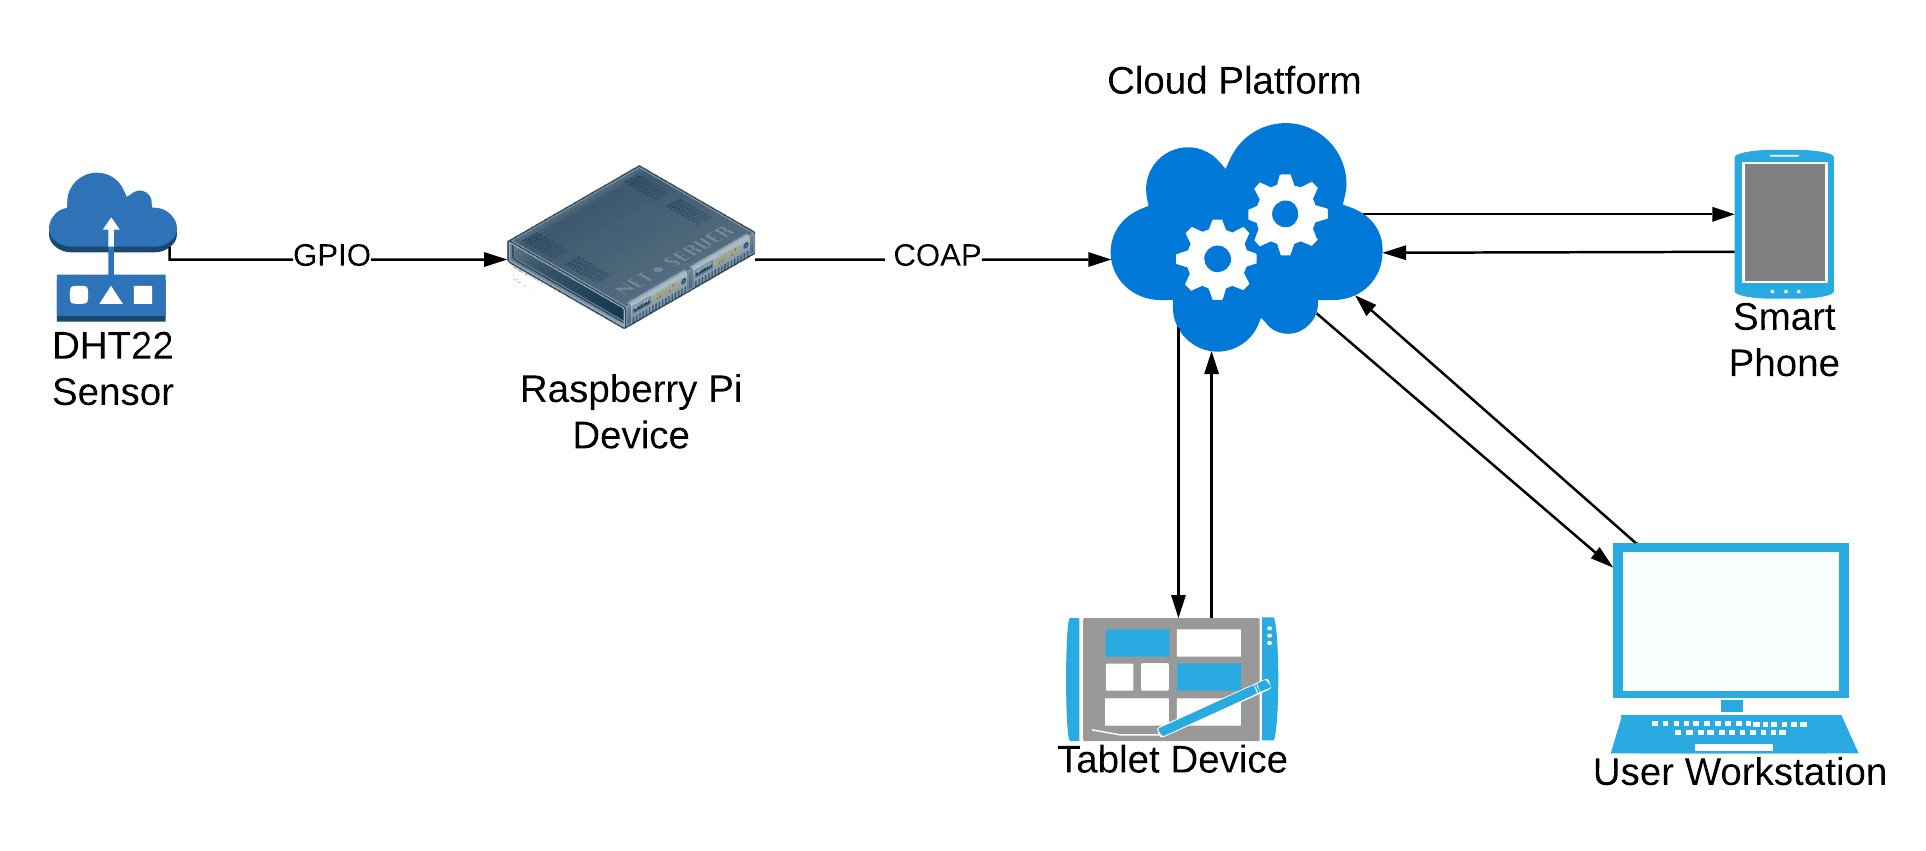
\includegraphics[width=1\textwidth]{assets/Project_Framework.png}}
    \caption{\label{fig:proj_framework} The project infrastructure.}
\end{figure}


The DHT22 sensor will connect to the \gls{rpi} using the \gls{rpi}'s on board 
\gls{gpio} ports as shown in \figref{fig:rpi_wiring}. 
Using the AdaFruit Python DHT library, a library that provides methods to interact 
with DHT sensors connected to the \gls{rpi}'s \gls{gpio} pins, 
and the CoAPthon library, a Python implementation of the \gls{coap} protocol, a 
Python script will create a \gls{coap} endpoint.
This endpoint will act as an \gls{api} for the DHT 22 sensor. 
The script will use the AdaFruit DHT methods to get the DHT 22 sensors temperature 
and humidity data. This data will then be formatted into \gls{json} in order to 
be transmitted. Then using the CoAPthon library a \gls{coap} message will be created 
with the sensors \gls{json} data as the payload. This message will then be sent over
\gls{udp} to a \gls{coap} \gls{uri} hosted by the cloud platform. The cloud endpoint 
will receive the \gls{json} data, format it and display it to the user, who will 
be accessing the cloud platform via \gls{http}. This process is shown in \algref{alg:get_send_data_alg}.

\begin{center}
\begin{algorithm}[H]
    \KwData{Temperature and humidity data from sensor}
    \KwResult{Sensor data sent to Cloud CoAP endpoint}
    initialization\;
    define interval in seconds (DHT 22 sensor interval is 2 seconds)\;
    \While{running}{
        get latest sensor data from DHT 22 sensor\;
        \eIf{sensor data is returned}{
            format data into json object\;
            create CoAP Post message with cloud uri as destination\;
            send CoAP message\;
        }{
            wait interval time and continue\;
        }
    }
    \caption{\label{alg:get_send_data_alg}How to get data from sensor and send to cloud.}
\end{algorithm}
\end{center}

\begin{figure}[H]
    \centering
    \makebox[1\textwidth]{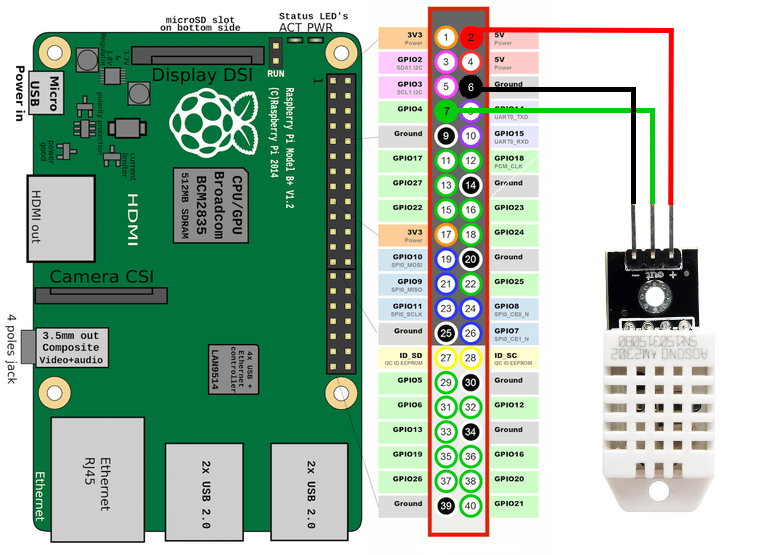
\includegraphics[width=1\textwidth]{assets/rpi_wiring.png}}
    \caption{\label{fig:rpi_wiring} Wiring diagram for connecting the sensor to the \gls{rpi}.}
\end{figure}